\documentclass{article}

\usepackage{fancyhdr}
\usepackage{ragged2e}
\usepackage{graphicx}
\usepackage{caption}
\usepackage{geometry}
\usepackage{amsmath}
\usepackage{rotating}

\usepackage{listings}
\usepackage{color}

\definecolor{dkgreen}{rgb}{0,0.6,0}
\definecolor{gray}{rgb}{0.5,0.5,0.5}
\definecolor{mauve}{rgb}{0.58,0,0.82}

\lstset{frame=tb,
  language=Java,
  aboveskip=3mm,
  belowskip=3mm,
  showstringspaces=false,
  columns=flexible,
  basicstyle={\small\ttfamily},
  numbers=none,
  numberstyle=\tiny\color{gray},
  keywordstyle=\color{blue},
  commentstyle=\color{dkgreen},
  stringstyle=\color{mauve},
  breaklines=true,
  breakatwhitespace=true,
  tabsize=4
}

\setcounter{secnumdepth}{1}

\usepackage{chngcntr}
\counterwithin{figure}{section}

\renewcommand*{\thepage}{C\arabic{page}}

\pagestyle{fancy}
\lhead{ACME Robotics}
\chead{\#8367}
\rhead{\ifcontents Contents \else Week \thesection \fi}

\newif\ifcontents
\contentsfalse

\makeatletter
\renewcommand{\@seccntformat}[1]{}
\makeatother

\begin{document}

\subsection{Write code to identify the position of the jewels using vision}
%!Use OpenCV and basic image processing to reliably determine the state of the jewels during autonomous.
Ryan worked on a basic jewel vision system. Although the actual algorithm/image processing is simple, there's a lot of ``glue'' code necessary to get vision working properly. During the 24-hour build, Ryan was able to download and add OpenCV to the Android project, and, after some frustrating debugging, he was able to convert Vuforia preview frames into OpenCV mats. Ryan used this code to get OpenCV images from the Vuforia preview. Specific regions from the jewel were then cropped out of the image and used to compute the average RGB color. Here's the code for computing the red/blue color ratios:
\begin{lstlisting}[language=Java]
Mat leftJewelCropped = rgb.submat(leftJewelRect);
Mat rightJewelCropped = rgb.submat(rightJewelRect);

Scalar leftJewelTotalColor = Core.sumElems(leftJewelCropped);
Scalar rightJewelTotalColor = Core.sumElems(rightJewelCropped);

leftBlue = leftJewelTotalColor.val[0];
leftRed = leftJewelTotalColor.val[2];
rightBlue = rightJewelTotalColor.val[0];
rightRed = rightJewelTotalColor.val[2];

double leftTotal = leftBlue + leftRed;
double rightTotal = rightBlue + rightRed;

if (leftTotal == 0) {
    leftBlue = 0;
    leftRed = 0;
} else {
    leftBlue /= leftTotal;
    leftRed /= leftTotal;
}

if (rightTotal == 0) {
    rightBlue = 0;
    rightRed = 0;
} else {
    rightBlue /= rightTotal;
    rightRed /= rightTotal;
}
\end{lstlisting}

This can then be easily converted into a binary red/blue or blue/red jewel configuration output. The next bit of glue code involves superimposing an overlay on top of the preview and drawing the jewel rects with the appropriate color. This was actually the most difficult part of the whole thing; it took many tries to get the canvas transforms working properly. However, in the end, everything went together nicely and was able to accurately assess the jewel colors. Michael, Kelly, and Ryan also tested it briefly in different lighting conditions and it worked flawlessly. Figure \ref{fig:vision} shows a screenshot of the end result.
\begin{figure}[h]
    \centering
    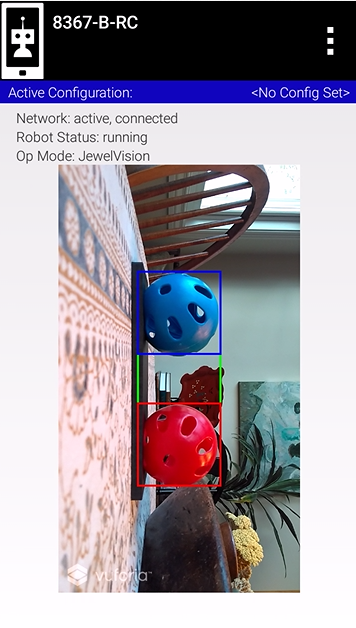
\includegraphics[width=.6\textwidth,height=3in,keepaspectratio]{02/images/jewelvision.PNG}
    \caption{Caption}
    \label{fig:vision}
\end{figure}

\subsection{Setup version control and task tracking and explain the general software workflow to new members}
%!Setup a new repo on GitHub for this season, with the task tracker we will be using, Jira, and continuous integration. Explain the software workflow with Git and Jira to the new software members.
Ryan setup a new Android Studio project with the SDK in a separate directory. He also copied some of the necessary files from previous seasons and added CI. Michael also introduced Jira to the team. The team decided that some kind of issue tracking functionality would help organize the software tasks, especially between multiple people. They also decided to have a more well-defined, systematic procedure for integrating changes. For the most part, new features will be created in separate branches corresponding to issues in Jira. Once the changes are ready, a pull request will be created and the code will be reviewed before finally be merged into the master branch. Overall, this workflow keeps the master branch clean and operational (in theory) and the whole repo structurally better. 

\subsection{Write dead reckoning code for localizing the robot.}
%!Use data from only the encoders and gyro to determine the position of the robot on the field, for executing path and placing glyphs.
Kelly worked on dead reckoning code. When location cannot be determined by vison, either Vuforia or some sort of cryptobox detection, the position of the robot can be estimated by measuring movements using internal sensors (encoders on the drive motors and the gyro), and keeping track of the robots movement from the last known position. When working with a tank drive style drive base, it is best to assume that each incremental movement that is being measured is in an arc, rather than a straight line, in order to reduce error. The average displacement of all drive motor encoders is used to determine the distance the robot has travelled, and then the angular displacement is measured from the gyro, this is shown in figure \ref{fig:twist}. When the arc length and angle are known, the radius and chord length of the arc can be calculated, using $$r=\frac{l_{arc}}{\theta}$$ $$l_{chord} = r \sqrt{2(1-\cos{\theta})}$$. The motion of the robot can then be represented in polar coordinates, theta is equal to the final heading of the robot, and r is equal to the chord length. It is then easy to convert to cartesian coordinates and find the updated position of the robot.
\begin{figure}[h]
    \centering
    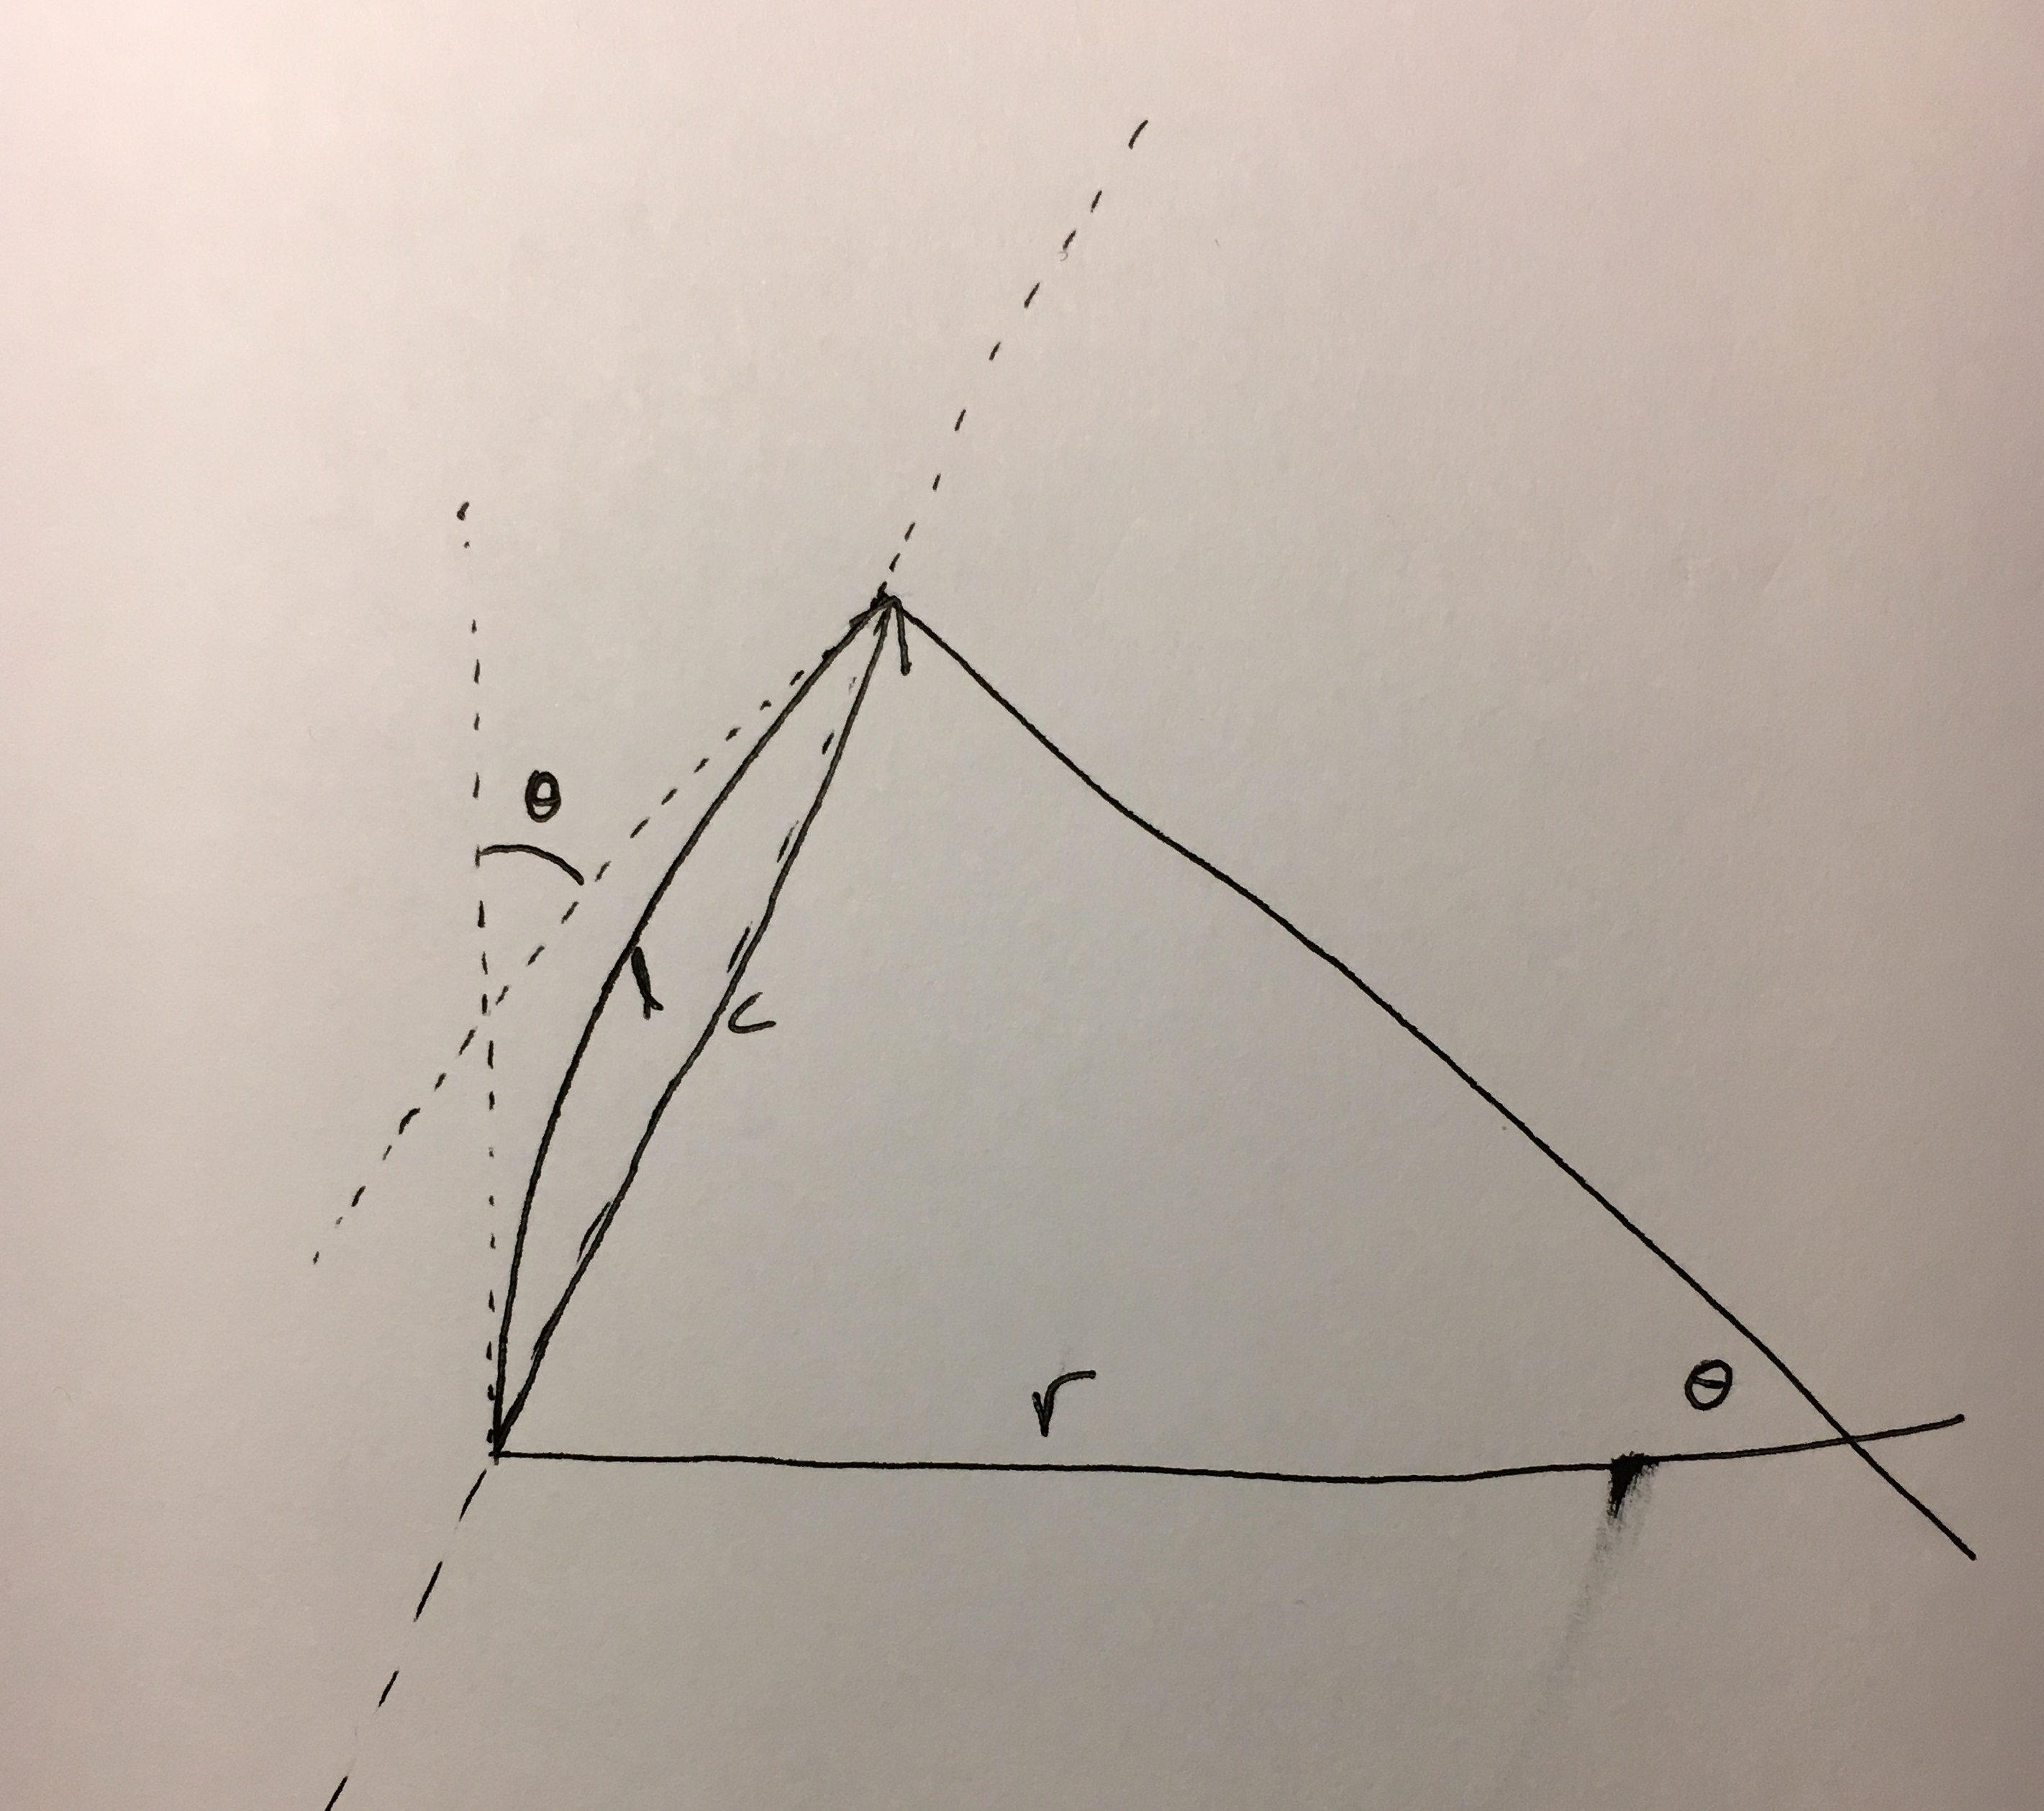
\includegraphics[width=.6\textwidth]{02/images/twist.jpg}
    \caption{Caption}
    \label{fig:twist}
\end{figure}

\end{document}